% 图 3.2 晶体场配位多面体：(a) 八面体配位 (b) 四面体配位（立方体内接四面体）
\documentclass[tikz,border=5pt]{standalone}
\usetikzlibrary{arrows.meta}
\usepackage{amsmath}
\usepackage{bm}
\usepackage{fontspec}
\setmainfont{Times New Roman}
\begin{document}
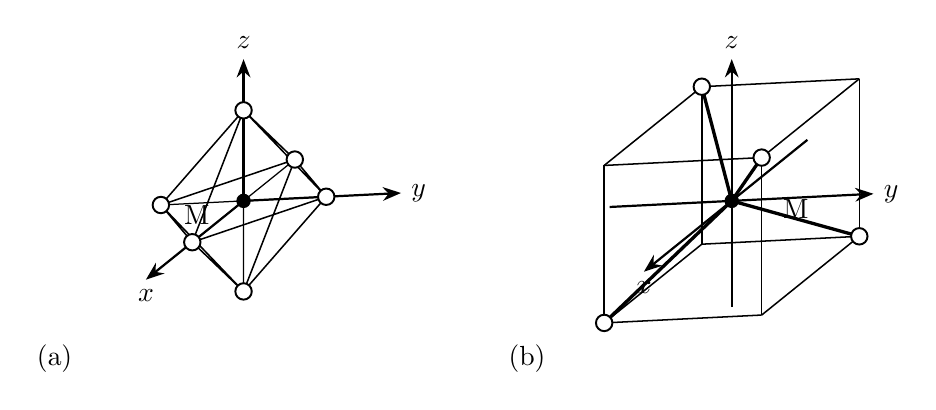
\begin{tikzpicture}[line width=0.8pt,>=Stealth]
% ---------- (a) octahedron ----------
\begin{scope}[x={(-0.62cm,-0.50cm)},y={(1cm,0.05cm)},z={(0,1cm)}]
% axes
\draw[->] (0,0,0) -- (0,0,1.8) node[above]{$z$};
\draw[->] (0,0,0) -- (0,2.0,0) node[right]{$y$};
\draw[->] (0,0,0) -- (2.0,0,0) node[below]{$x$};
% octahedron edges
\draw[line width=0.55]
  (0,0,1.15) -- (0,1.05,0)   (0,0,1.15) -- (1.05,0,0)
  (0,0,1.15) -- (0,-1.05,0)  (0,0,1.15) -- (-1.05,0,0)
  (0,0,-1.15) -- (0,1.05,0)  (0,0,-1.15) -- (1.05,0,0)
  (0,0,-1.15) -- (0,-1.05,0) (0,0,-1.15) -- (-1.05,0,0)
  (0,1.05,0) -- (1.05,0,0)   (1.05,0,0) -- (0,-1.05,0)
  (0,-1.05,0) -- (-1.05,0,0) (-1.05,0,0) -- (0,1.05,0);
% spokes M -> vertices
\draw[line width=0.45]
  (0,0,0) -- (0,0,1.15)  (0,0,0) -- (0,0,-1.15)
  (0,0,0) -- (0,1.05,0)  (0,0,0) -- (0,-1.05,0)
  (0,0,0) -- (1.05,0,0)  (0,0,0) -- (-1.05,0,0);
% ligand balls and central ion
\node[circle,draw,fill=white,inner sep=2.1pt,line width=0.7] at (0,0,1.15) {};
\node[circle,draw,fill=white,inner sep=2.1pt,line width=0.7] at (0,0,-1.15) {};
\node[circle,draw,fill=white,inner sep=2.1pt,line width=0.7] at (0,1.05,0) {};
\node[circle,draw,fill=white,inner sep=2.1pt,line width=0.7] at (0,-1.05,0) {};
\node[circle,draw,fill=white,inner sep=2.1pt,line width=0.7] at (1.05,0,0) {};
\node[circle,draw,fill=white,inner sep=2.1pt,line width=0.7] at (-1.05,0,0) {};
\fill (0,0,0) circle (2.6pt);
\node[anchor=east,inner sep=2pt] at (0.56,0,0.10) {$\mathrm{M}$};
\end{scope}
\node at (-2.4,-2.0) {(a)};
% ---------- (b) cube + tetrahedron ----------
\begin{scope}[shift={(6.2,0)},x={(-0.62cm,-0.50cm)},y={(1cm,0.05cm)},z={(0,1cm)}]
% axes
\draw[->] (0,0,-1.35) -- (0,0,1.8) node[above]{$z$};
\draw[->] (0,-1.55,0) -- (0,1.8,0) node[right]{$y$};
\draw[->] (-1.55,0,0) -- (1.8,0,0) node[below]{$x$};
% cube edges
\foreach \a in {-1,1}{\foreach \b in {-1,1}{
  \draw[line width=0.55] (\a,\b,-1) -- (\a,\b,1);
  \draw[line width=0.55] (\a,-1,\b) -- (\a,1,\b);
  \draw[line width=0.55] (-1,\a,\b) -- (1,\a,\b);
}}
% tetrahedron: bold spokes to alternate corners
\draw[line width=1.2] (0,0,0) -- (1,1,1);
\draw[line width=1.2] (0,0,0) -- (1,-1,-1);
\draw[line width=1.2] (0,0,0) -- (-1,1,-1);
\draw[line width=1.2] (0,0,0) -- (-1,-1,1);
% ligand balls on tetrahedron corners, central ion
\node[circle,draw,fill=white,inner sep=2.1pt,line width=0.7] at (1,1,1) {};
\node[circle,draw,fill=white,inner sep=2.1pt,line width=0.7] at (1,-1,-1) {};
\node[circle,draw,fill=white,inner sep=2.1pt,line width=0.7] at (-1,1,-1) {};
\node[circle,draw,fill=white,inner sep=2.1pt,line width=0.7] at (-1,-1,1) {};
\fill (0,0,0) circle (2.6pt);
\node[anchor=west,inner sep=2pt] at (-0.35,0.35,-0.30) {$\mathrm{M}$};
\end{scope}
\node at (6.2-2.6,-2.0) {(b)};
\end{tikzpicture}
\end{document}
